% -------------------------------
% Plantilla del TFG en la ESIIAB-UCLM. Versión 0.0 (Preliminar)
%
% Luis de la Ossa
% 
% Compilar con XeLaTeX 
% -------------------------------
\documentclass[12pt, a4paper]{book}

% -------------------------------
% Información y opciones del documento. Debe editarse.
% -------------------------------
% -------------------------------
% Plantilla del TFG en la ESIIAB-UCLM. Versión 0.0 (Preliminar)
%
% Luis de la Ossa
% 
% Compilar con XeLaTeX 
% -------------------------------


% -------------------------------
% Comandos comunes
% -------------------------------
\newcommand{\uclm}{University of Castilla-La Mancha\,}
\newcommand{\dsi}{Computing Systems Department\,}
\newcommand{\esii}{School of Computer Science and Engineering\,}


% -------------------------------
% Comandos específicos
% -------------------------------
\newcommand{\autor}{Student's name\,}
\newcommand{\titulo}{Dissertation title \,}
\newcommand{\director}{Supervisor's name\,}
\newcommand{\codirector}{Co-Supervisor's name\,}
\newcommand{\fecha}{May, 2020\,}
 \newcommand{\espec}{ \quad \ldots \quad \,} 







% -------------------------------
% Configuración del documento, paquetes, etc. 
% -------------------------------
% -------------------------------
% Plantilla del TFG en la ESIIAB-UCLM. Versión 0.0 (Preliminar)
%
% Luis de la Ossa
% 
% Compilar con XeLaTeX 
% -------------------------------


% -------------------------------
% Idioma
% -------------------------------
\usepackage{polyglossia}
%\setmainlanguage{spanish}


% -------------------------------
% Fuente
% -------------------------------
% Cualquier tamaño de texto: {\fontsize{100pt}{120pt}\selectfont tutexto}
\usepackage{anyfontsize}
% Selección de fuentes.
\usepackage{fontspec}
% Espacio entre líneas
\usepackage{setspace}
% Fuentes especiales
\usepackage{textcomp,marvosym,pifont}


% -------------------------------
% Otros paquetes de uso común
% -------------------------------
% Símbolos matemáticos
\usepackage{amsmath,amsfonts,amssymb}
% Gráficos
\usepackage{graphicx}
% Posición arbitraria de los gráficos
\usepackage[absolute,overlay]{textpos}
% Apéndices
\usepackage{appendix}


% -------------------------------
% Esquema de colores
% -------------------------------
% Paquete para la definición de colores
\usepackage[table]{xcolor}
% Esquema de colores
% -------------------------------
% Plantilla del TFG en la ESIIAB-UCLM. Versión 0.0 (Preliminar)
%
% Luis de la Ossa
% 
% Compilar con XeLaTeX 
% -------------------------------

% -------------------------------
% Color del tema
% -------------------------------

% Color para los títulos, etc.
%\definecolor{tema}{RGB}{0,0,0}        % Negro 
%\definecolor{tema}{RGB}{182,0,52}     % LOGO UCLM
\definecolor{tema}{RGB}{0,69,134}      % Azul del esquema  
%\definecolor{tema}{RGB}{197,0,11}     % Rojo del esquema     

% Negritas con el color del tema
\newcommand{\bft}[1]{\textcolor{tema}{\bf #1}} 


% -------------------------------
% Esquema de colores
% -------------------------------
% Estos balores coinciden con colores de OpenOffice 
% Se pueden redefinir para que coincidan con las paletas de las 
% herramientas utilizadas para hacer las gráficas.
\definecolor{blanco}{RGB}{255,255,255} 
\definecolor{negro}{RGB}{0,0,0}
\definecolor{gris95}{gray}{.95}
\definecolor{gris75}{gray}{.75}
\definecolor{gris50}{gray}{.50}
\definecolor{gris25}{gray}{.25}
\definecolor{rojo}{RGB}{197,0,11}        % Gráfico 11
\definecolor{azul}{RGB}{0,69,134}        % Gráfico 1
\definecolor{verde}{RGB}{87,157,28}      % Gráfico 4
\definecolor{naranja}{RGB}{255, 149, 14} % Gráfico 10
\definecolor{mostaza}{RGB}{255, 211, 32} % Gráfico 3

% Negrita con color definido 
\newcommand{\bfa}[1]{\textcolor{azul}{\bf #1}} 
\newcommand{\bfr}[1]{\textcolor{rojo}{\bf #1}}
\newcommand{\bfn}[1]{\textcolor{naranja}{\bf #1}}
\newcommand{\bfv}[1]{\textcolor{verde}{\bf #1}}  
\newcommand{\bfm}[1]{\textcolor{mostaza}{\bf #1}} 






% -------------------------------
% Márgenes
% -------------------------------
% Márgenes de las páginas
\usepackage[
  inner	 =	3cm,   % Margen interior
  outer	 =	2.5cm, % Margen exterior
  top	 =	2.5cm, % Margen superior
  bottom =	2.5cm, % Margen inferior
  includeheadfoot, % Incluye cabecera y pie de página en los márgenes
]{geometry}
% Muestra una regla para comprobar el formato de las páginas (descomentar)
%\usepackage[type=upperleft,showframe,marklength=8mm]{fgruler} 


% -------------------------------
% Renombra tablas y bibliografía
% -------------------------------
%\addto\captionsspanish{
%	\renewcommand{\listtablename}{Índice de tablas} 
%	\renewcommand{\tablename}{Tabla}
%	\renewcommand{\bibname}{Referencia bibliográfica}
%}


% -------------------------------
% Itemize y enumerate. Control de los espacios.
% -------------------------------
\usepackage{enumitem}
\setitemize{itemsep=0pt}
\setenumerate{itemsep=0pt}
\renewcommand{\labelitemi}{\tiny\bft{$\blacksquare$}}
\renewcommand{\labelitemii}{\bft{$\bullet$}}
\renewcommand{\labelitemiii}{\bft{-}}


% -------------------------------
% Enlaces y colores
% -------------------------------
\usepackage{hyperref}
%\hypersetup{
%    colorlinks,
%    citecolor=black,
%    filecolor=black,
%    linkcolor=black,
%    urlcolor=black
%}

% -------------------------------
% Gestión de elementos flotantes
% -------------------------------
% Para forzar a que las figuras aparezcan antes del fin de una sección.
%\usepackage[section]{placeins}

% Gestión de títulos de los elementos flotantes
\usepackage{caption}
% Subfiguras y títulos en subfiguras
\usepackage{subcaption}

% Títulos
\DeclareCaptionFont{tema}{\color{tema}} % Color
\captionsetup{labelfont={tema, bf}}     % Estilo
\captionsetup{font=normalsize}          % Tamaño
\captionsetup{width=.9\linewidth}       % Anchura del título
 % Distancia de la figura al texto.
\setlength{\intextsep}{1cm} 
\setlength{\textfloatsep}{1cm}         
       

% -------------------------------
% Utilidades para tablas
% -------------------------------
% Para fundir filas en tablas
\usepackage{multirow}
% Para definir columnas con ancho fijo y alineación
\usepackage{array,ragged2e}
\newcolumntype{L}[1]{>{\raggedright\let\newline\\\arraybackslash\hspace{0pt}}m{#1}}
\newcolumntype{C}[1]{>{\centering\let\newline\\\arraybackslash\hspace{0pt}}m{#1}}
\newcolumntype{R}[1]{>{\raggedleft\let\newline\\\arraybackslash\hspace{0pt}}m{#1}}


% -------------------------------
% Para tabular
% -------------------------------
\usepackage{tabto}


% -------------------------------
% Formato de títulos, capítulos, etc.
% -------------------------------
\usepackage{titlesec, titletoc}
% Parte
\titleformat{\part}[display]												   	   % Estilo
	{\Huge \centering \color{tema}}                                                % Formato
	{Parte \thepart }                                                              % Etiqueta
	{0.75ex}                                                                       % Separación
	{\bfseries\fontsize{25pt}{40pt}\selectfont}                                    % Entre etiqueta y título            
	[\thispagestyle{empty}]                                                        % Después

% Capítulo		
\titleformat{\chapter}[block]            			 			                    % Estilo  	
	{\vspace{0cm} \flushright \bfseries \LARGE \color{tema}}  	        			% Formato 
	{\thechapter.}                  			  									% Etiqueta
	{0.75ex}                                     									% Separación
	{}                                           									% Entre etiqueta y título
	[\vspace{0.1cm} \rule{0.5\textwidth}{1pt}\vspace*{1cm}\thispagestyle{plain}]    % Después      
  
% Sección
\titleformat{\section}
	{\vspace{5pt}  \Large \color{tema}}
	{\thesection .}
	{0.75ex}
	{}

% Subsección
\titleformat{\subsection}
	{\large \color{tema}}
	{\thesubsection .}
	{0.75ex}
	{}
 
% Subsubsección
\titleformat{\subsubsection}
	{\bf\color{tema}}
	{}
	{0.75ex}
	{}
	 
% Parte (TOC)
\titlecontents{part}[2pc]
  	{\vspace{20pt}\bfseries\filright\Large\color{tema}}
  	{\contentslabel{1.5pc}}{\hspace*{-1.5pc}}
  	{\vspace{5pt}}
  	{}
  
% Capítulo (TOC)
\titlecontents{chapter}[2pc]
  	{\vspace{10pt}\bfseries\large\filright}
  	{\contentslabel{1.5pc}}{\hspace*{-1.5pc}}
  	{\mdseries\titlerule*[0.5pc]{.}\bfseries\contentspage}

% Sección (TOC)
\titlecontents{section}[4pc]
  	{\vspace{5pt}\filright}
  	{\contentslabel{2pc}}{\hspace*{2pc}}
  	{\titlerule*[0.5pc]{.}\contentspage}
  	{\vspace{5pt}

% Subsección (TOC)
\titlecontents{subsection}[6pc]
  	{\vspace{2.5pt}\filright\small\em}
  	{\contentslabel{3pc}}{\hspace*{-3pc}}
  	{\titlerule*[0.5pc]{.}\contentspage} 
  	
  	
% -------------------------------
% Cabeceras y pie de página
% -------------------------------
\usepackage{fancyhdr}
\pagestyle{fancy}
\fancyhf{}

% Permite incluir la parte. Para ello crea \parttitle
\let\Oldpart\part
\newcommand{\parttitle}{}
\renewcommand{\part}[1]{\Oldpart{#1}\renewcommand{\parttitle}{#1}}

% Cabeceras y pies de página
\fancyhead[LE]{}
\fancyhead[RO]{\slshape \leftmark}
\fancyfoot[LE,RO]{\thepage}
\renewcommand{\footrulewidth}{1pt}
\renewcommand{\headrulewidth}{1pt}
\renewcommand{\chaptermark}[1]{\markboth{#1}{}} % Capítulo (Solo texto)
\renewcommand{\chaptermark}[1]{\markboth{\thechapter. #1}{}} % Capítulo (Número y texto)

% Formato plano para las páginas con títulos (solo incluye el pie de página)
\fancypagestyle{plain}{
\fancyhf{}
\fancyhead{}
\fancyfoot[LE,RO]{\thepage}
\renewcommand{\footrulewidth}{1pt}
\renewcommand{\headrulewidth}{0pt}
}

 
% -------------------------------
% Utilidades
% -------------------------------
% Marcas
\newcommand{\pcite}{\bfr{\large[?]}\,} % Cita pendiente: [?] en rojo y negrita.
\newcommand{\ps}{\bfr{\huge[--}\,} % Pricipio de un bloque en sucio
\newcommand{\fs}{\bfr{\huge--]}\,} % Fin de un bloque en sucio.

% Notas
\usepackage[textsize=tiny,spanish,shadow,textwidth=2cm]{todonotes}

% Para generar textos "random"
\usepackage{lipsum} 
 

% -------------------------------
% Algoritmos y código
% -------------------------------

% Se definen entornos específicos para algoritmos y código que permiten
% gestionar los títulos manera similar en ambos casos, y similar al resto
% de elementos flotantes.
\usepackage{newfloat}

\DeclareFloatingEnvironment[ % Algoritmos
  listname = {List of Algorithms},
  name = Algorithm
]{algorithm}

\DeclareFloatingEnvironment[ % Fragmentos de código
  listname = {List of Code Listings},
  name = {Code listing}
]{code}

% Define un estilo para el encabezado de algoritmos y código.
\DeclareCaptionFormat{algcode}{
% OPCIÓN 1 -> Línea debajo del título
\rule{\dimexpr\textwidth\relax}{0.4pt}\vspace{0cm}
#1#2#3
\vspace{-0.2cm}\rule{\dimexpr\textwidth\relax}{0.4pt} % 
% OPCIÓN 2 -> Sin línea debajo del título
%\rule{\dimexpr\textwidth\relax}{0.4pt}\vspace{0cm}
%#1#2#3
}
\captionsetup[algorithm]{format=algcode, width=\linewidth}
\captionsetup[code]{format=algcode, width=\linewidth}

% Opciones específicas para algoritmos.
\usepackage[noend]{algpseudocode}
% Tamaño de letra y separadores
\makeatletter
\renewcommand{\ALG@beginalgorithmic}{\small\hrule\vskip10pt}
\makeatother
% Variables y funciones
\newcommand{\va}[1]{{\it {#1}}}				
\newcommand{\fu}[1]{{\textsc{#1}}}          
% Palabras clave
\renewcommand{\algorithmicrepeat}{\bft{repetir}}
\renewcommand{\algorithmicuntil}{\bft{hasta}}
\renewcommand{\algorithmicend}{\bft{fin}}
\renewcommand{\algorithmicif}{\bft{si}}
\renewcommand{\algorithmicthen}{\bft{entonces}}
\renewcommand{\algorithmicelse}{\bft{si no}}
\newcommand{\algorithmicelsif}{\algorithmicelse\ \algorithmicif}
\newcommand{\algorithmicendif}{\algorithmicend\ \algorithmicif}
\renewcommand{\algorithmicfor}{\bft{para}}
\renewcommand{\algorithmicforall}{\bft{para cada}}
\renewcommand{\algorithmicwhile}{\bft{mientras}}
\renewcommand{\algorithmicdo}{\bft{hacer}}
\renewcommand{\algorithmicprocedure}{\bft{procedimiento}}
\renewcommand{\algorithmicreturn}{\bft{devolver}}
\renewcommand{\algorithmicfunction}{\bft{función}}
\renewcommand{\algorithmicloop}{\bft{iterar}}

% Opciones específicas para código.
\usepackage{listings}
% Aspecto de los listados de código (ejemplo)
% Los colores se han de cambiar y adaptar a los distintos lenguajes de programación.
\lstset{
    language=Python,
    keywordstyle=\bf\color{tema},  
	breaklines=true,    
	basicstyle={\small\ttfamily},
    tabsize=5,
    frame=t % Es importante no cambiar esta opción (es la línea superior) 
}

% -------------------------------
% Cacacteres pifont de uso común (con color)
% -------------------------------
\newcommand{\vmarkt}{\textcolor{tema}{\ding{52}} }  % Checked (V) Tema
\newcommand{\vmarkr}{\textcolor{rojo}{\ding{52}} }  % Checked (V) Rojo
\newcommand{\vmarka}{\textcolor{azul}{\ding{52}} }  % Checked (V) Azul

\newcommand{\xmarkt}{\textcolor{tema}{\ding{55}} }  % Checked (X) Tema
\newcommand{\xmarkr}{\textcolor{rojo}{\ding{55}} }  % Checked (X) Rojo
\newcommand{\xmarka}{\textcolor{azul}{\ding{55}} }  % Checked (X) Azul

\newcommand{\lmarkt}{\textcolor{tema}{\ding{46}} }  % Lápiz Tema
\newcommand{\lmarkr}{\textcolor{rojo}{\ding{46}} }  % Lápiz Rojo
\newcommand{\lmarka}{\textcolor{azul}{\ding{46}} }  % Lápiz Azul

\newcommand{\hmarkt}{\textcolor{tema}{\ding{43}} }  % Mano Tema
\newcommand{\hmarkr}{\textcolor{rojo}{\ding{43}} }  % Mano Roja 
\newcommand{\hmarka}{\textcolor{azul}{\ding{43}} }  % Mano Azula 

\newcommand{\fmarkt}{\textcolor{tema}{\ding{220}} }  % Flechza Tema
\newcommand{\fmarkr}{\textcolor{rojo}{\ding{220}} }  % Flecha Roja 
\newcommand{\fmarka}{\textcolor{azul}{\ding{220}} }  % Flecha Azul

% Documento
\begin{document}

% -------------------------------
% Portada y título
% -------------------------------
% Fuente  de la portada
% \setmainfont[Ligatures={NoRequired,NoCommon,NoContextual}]{Calibri}
% -------------------------------
% Plantilla del TFG en la ESIIAB-UCLM. Versión 0.0 (Preliminar)
%
% Luis de la Ossa
% 
% Compilar con XeLaTeX 
% -------------------------------
\pagestyle{empty}
\begin{titlepage}\null



\begin{textblock*}{\paperwidth}(0cm,3cm)
\begin{center}

\includegraphics[width=4cm]{figs/logoconciti.png}
\end{center}
\end{textblock*}


\begin{textblock*}{\paperwidth}(0cm,8cm) 
\begin{center}\doublespacing
{\fontsize{16pt}{2pt}\selectfont \uclm}

{\fontsize{16pt}{2pt}\selectfont \esii}
\end{center}
\end{textblock*}


\begin{textblock*}{\paperwidth}(0cm,12cm) 
\begin{center}\doublespacing 
{\bf\fontsize{18pt}{4pt}\selectfont Undergraduate Dissertation}

{\fontsize{18pt}{4pt}\selectfont Bachelor's Degree in Computer Science and Engineering}

{\fontsize{16pt}{4pt}\selectfont Major in \quad \ldots \quad}
\end{center}
\end{textblock*}


% El título ocupa el 80% de la página. Puede adaptarse 
% a la longitud del texto
\begin{textblock*}{0.8\paperwidth}(0.1\paperwidth,17.5cm) 
\begin{center}\doublespacing % onehalfspace
{\bf\fontsize{20pt}{4pt}\selectfont \titulo}

\vskip1cm
{\it \fontsize{18pt}{4pt}\selectfont \autor}
\end{center}
\end{textblock*}


\begin{textblock*}{\paperwidth}(0cm,25.5cm) 
\begin{center}
{\fontsize{14pt}{4pt}\selectfont \fecha}
\end{center}
\end{textblock*}
\end{titlepage}

% -------------------------------
% Fuente del documento.
% -------------------------------
\setmainfont[Ligatures={NoRequired,NoCommon,NoContextual}]{Calibri}

% -------------------------------
% Preámbulo
% -------------------------------
\frontmatter 
% -------------------------------
% Plantilla del TFG en la ESIIAB-UCLM. Versión 0.0 (Preliminar)
%
% Luis de la Ossa
% 
% Compilar con XeLaTeX 
% -------------------------------


% -------------------------------
% Segunda portada
% -------------------------------
\cleardoublepage
\setcounter{page}{1} \null

\begin{textblock*}{3cm}(3cm,2cm) 
\begin{flushleft}

\includegraphics[height=2cm]{figs/logouclm.png}
\end{flushleft}
\end{textblock*}


\begin{textblock*}{2.5cm}(15.95cm,2.45cm) 
\begin{flushright}

\includegraphics[height=1.4cm]{figs/euroinf.jpg}
\end{flushright}
\end{textblock*}

\begin{textblock*}{2cm}(14cm,2cm)  % Corrige la posición porque la imagen tiene margen
\begin{flushright}

\includegraphics[height=2cm]{figs/logoesii.png}
\end{flushright}
\end{textblock*}



\begin{textblock*}{\textwidth}(3cm,8cm) 
\begin{center}\doublespacing 
{\fontsize{18pt}{4pt}\selectfont \bft{UNDERGRADUATE DISSERTATION}}

\medskip
{\fontsize{18pt}{4pt}\selectfont Bachelor's Degree in Computer Science and Engineering}

\medskip
{\fontsize{16pt}{4pt}\selectfont Major in \espec}
\end{center}
\end{textblock*}


\begin{textblock*}{\textwidth}(3cm,14cm) 
\begin{center}\doublespacing 
{\fontsize{22pt}{4pt}\selectfont \bft{\titulo}}
\end{center}
\end{textblock*}


\begin{textblock*}{\textwidth}(3cm,20.5cm) 
\begin{flushleft}\doublespacing
{\fontsize{14pt}{4pt}\selectfont \bft{Author:} \autor}

{\fontsize{14pt}{4pt}\selectfont \bft{Supervisor:} \director}

{\fontsize{14pt}{4pt}\selectfont \bft{Co-Supervisor:} \codirector}
\end{flushleft}
\end{textblock*}


\begin{textblock*}{\linewidth}(3cm,25cm) 
\begin{flushright}
{\fontsize{14pt}{4pt}\selectfont \fecha}
\end{flushright}
\end{textblock*}


% -------------------------------
% Dedicatoria
% -------------------------------
\cleardoublepage
\thispagestyle{empty}

\vspace*{9cm}  
\begin{flushright} \em 
Aquí va la dedicatoria que cada cual \\ 
quiera escribir. El ancho se controla \\ 
manualmente
\end{flushright}


% -------------------------------
% Declaración de autoría
% -------------------------------
\cleardoublepage
\thispagestyle{plain}
\begin{center}
\Large{\bft{Autorship Statement}}
\end{center}
\vskip1cm

I, the undersigned, \quad \ldots \quad, with ID number \quad \ldots \quad, declare that I am the sole author of the Undergraduate Dissertation titled ``\quad \ldots \quad '', that this work does not break the current intellectual property law. and that all the non-original material contained in this work is properly attributed to their legitimate authors.

\vspace*{2cm}
\begin{center}
Albacete, (date) 

\vskip3cm

Signed by: \autor
\end{center}


% -------------------------------
% Resumen
% -------------------------------
\cleardoublepage
\thispagestyle{plain}
\begin{center}
\Large{\bft{Abstract}}
\end{center}
\vskip1cm

\lipsum[1]

% -------------------------------
% Agradecimientos
% -------------------------------
\cleardoublepage
\thispagestyle{plain}
\begin{center}
\Large{\bft{Acknowledgements}}
\end{center}
\vskip1cm

\lipsum[1]

% -------------------------------
% Índices y tablas
% -------------------------------
\tableofcontents	% Índice
\listoffigures		% Índice de figuras
\listoftables		% Índice de tablas
\listofalgorithms   % Índice de algoritmos (comentar si no los hay)
\listofcodes	    % Índice de códigos (comentar si no los hay)
\cleardoublepage

% -------------------------------
% Documento
% -------------------------------
\mainmatter
% Estilo de página
\pagestyle{fancy}

% Introducción
\chapter{Aspect}
\lipsum[1-5]
\section{First section}
\lipsum[1-5]
\section{Second section}
\lipsum[1-5]
\subsection{Subsection}
\lipsum[1-6]

 

% Algunos elementos
\chapter{Some elements}

En este capítulo se describen algunas particularidades de la plantilla, y se proporcionan algunos ejemplos con elementos de uso frecuente. No se comentan aspectos comunes relacionados con el uso de \LaTeX, ya que existe gran cantidad de información al respecto.

\section{Configuration}
La configuración es muy sencilla. Al margen de la adaptación particular que pueda hacerse, la elaboración de un documento solamente requiere información relativa al autor, título y tutores. Ésta ha de configurarse en el archivo \verb+include\opciones.tex+.  \\

Además, en el archivo \verb+include\colores.tex+ puede configurarse el color \verb+tema+, utilizado en títulos, elementos flotantes y, opcionalmente, tablas y negritas. Por defecto, se recomienda ponerlo a \verb+{0,0,0}+  (negro). Pueden escribirse \bft{negritas con el color configurado} con el comando \verb+\bft{texto}+. \\

Por último, en el archivo principal se pueden configurar las fuentes utilizadas en la portada, preámbulo y documento.

\section{Colors}


En el archivo \verb+include\colores.tex+ se predefinen algunos colores. También varios comandos para utilizar negritas con ellos. En concreto, se proporcionan cinco: Con el comando \verb+\bfa{texto}+ se pueden poner las cosas en negrita \bfa{azul}. Con el comando \verb+\bfr{texto}+ se pueden poner las cosas en negrita \bfr{rojo}.Con el comando \verb+\bfn{texto}+ se pueden poner las cosas en negrita \bfn{naranja}. Con el comando \verb+\bfv{texto}+ se pueden poner las cosas en negrita \bfv{verde}. Con el comando \verb+\bfm{texto}+ se pueden poner las cosas en negrita \bfm{mostaza}.\\

\begin{itemize}
\item [\hmarkr] No es conveniente abusar los colores, salvo en alguna ocasión adicional. Por ejemplo, si el color del tema es {\bf negro} o \bfa{azul} se puede utilizar el \bfr{rojo} para alguna advertencia.
\end{itemize}

\section{Lists and enumerations}

El entorno \textit{itemize} usa, por defecto, el color del tema. Los símbolos utilizados para marcar los items están pre-definidos en el archivo de configuración, y pueden cambiarse. También es posible seleccionar, mediante \verb+\item[símbolo]+ el símbolo específico para cada línea. Esta lista muestra los símbolos por defecto:

\begin{itemize}
\item Primer ítem
\begin{itemize}
\item Primer ítem en el segundo nivel
\item Otro ítem en el segundo nivel
\begin{itemize}
\item Ítem en el tercer nivel
\end{itemize}
\end{itemize}
\item Segundo ítem
\item Tercer ítem \\
\end{itemize}

En esta se usan algunos caracteres especiales predefinidos para marcar los ítems. Existen comandos para mostrar algunos de estos caracteres con los colores azul, rojo y el color del tema.

\begin{itemize}
\item[\vmarka] \verb+\vmarka+ : ``v'' representa el símbolo, y ``a'' el color
\item[\xmarkr] \verb+\xmarkr+
\item[\lmarkt] \verb+\lmarkt+ : el color ``t'' corresponde al tema.
\item[\hmarkt] \verb+\hmarkt+ 
\item[\fmarkt] \verb+\fmarkt+ \\
\end{itemize}

Las enumeraciones también están preconfiguradas en el archivo de configuración:

\begin{enumerate}
\item Esto es una enumeración
\item Con algunos elementos adicionales
\item Que se pueden quitar
\end{enumerate}

Pueden ser modificadas, como en el siguiente ejemplo.

\begin{enumerate}[labelindent=\parindent ,leftmargin=*,label=\mbox{\bft{[Re \arabic*]}}]
\setcounter{enumi}{7}
\item Esto es una enumeración
\item Sin elementos
\item Adicionales
\end{enumerate}


\section{Floating elements}

En el archivo de \verb+include\configuracion+ existen varios parámetros que se fijan en la configuración para figuras y tablas, pero se pueden alterar de manera ocasional (y excepcional) al maquetar el documento. La mayoría son relativos al título, y se pueden cambiar a través de las funcionalidades que proporciona el paquete \verb+caption+. Cuando se cambian para un elemento particular \bft{es buena práctica restaurar el valor original}, para que el documento tenga un aspecto uniforme.

\begin{verbatim}
% Títulos
\DeclareCaptionFont{tema}{\color{tema}} % Color
\captionsetup{labelfont={tema, bf}}     % Estilo
\captionsetup{font=normalsize}          % Tamaño
\captionsetup{width=.9\linewidth}       % Anchura del título
 % Distancia de la figura al texto.
\setlength{\intextsep}{1cm} 
\setlength{\textfloatsep}{1cm}         
\end{verbatim}

\subsection{Tables}
Las tablas se hacen de modo normal, aunque se ha añadido la capacidad utilizar celdas que ocupen múltiples filas, colores en los encabezados, y anchuras fijas. Se recomienda mirar el código fuente de la tabla \ref{tab:mod1}.\\

Con respecto al color de los encabezados, es conveniente utilizar el mismo en todo el documento. Una opción con respecto al fondo del encabezado es utilizar el mismo que el del texto pero con transparencia. \\



% --------------------------------------------------
% Esto es para poner colores en las asignaturas
% en el ejemplo concreto
\newcommand{\bi}{\bfn{ES}/\bfr{EN}}
\newcommand{\esp}{\bfn{ES}}
\newcommand{\eng}{\bfr{EN}}
% --------------------------------------------------

\begin{table}[h]\footnotesize
\renewcommand{\arraystretch}{1.3} % Altura
\begin{center}
\begin{tabular}{|L{2.5cm}| L{3cm}| C{6cm} c | c |} % Tres primeras con anchura predefinida
\hline 
\rowcolor{tema!10} % Color con transparencia correspondiente
\bft{Módulo I} & \bft{Materia} & \multicolumn{2}{|c|}{\bft{Asignatura}}& \bft{ECTS} \\ \hline 

\multirow{9}{2.5cm}{Formación Básica (60 ECTS)} & % Aquí se indica que esta ocupa nueve filas.
\multirow{4}{3cm}{Fundamentos Matemáticos de la Informática} & 
Álgebra y Matemática Discreta & \esp  & 6 \\ \cline{3-5} 
& & Cálculo y Métodos Numéricos & \bi  & 6 \\ \cline{3-5} 
& & Estadística & \bi  & 6 \\ \cline{3-5}
& & Lógica& \esp  & 6 \\ \cline{2-5}
& Fundamentos Físicos de la Informática & Fundamentos Físicos de la Informática & \bi  & 6 \\ \cline{2-5}
& \multirow{2}{3cm}{Ingeniería de Computadores} & 
Estructura de Computadores & \esp  & 6 \\ \cline{3-5} 
& & Tecnología de Computadores & \esp  & 6 \\ \cline{2-5} 
& \multirow{2}{3cm}{Programación} & 
Fundamentos de Programación I & \esp  & 6 \\ \cline{3-5} 
& & Fundamentos de Programación II & \bi  & 6 \\ \cline{2-5}
%& \makecell[cl]{Gestión de las \\ Organizaciones} & Fundamentos de Gestión Empresarial & \esp  & 6 \\ \hline 
& Gestión de las \mbox{Organizaciones} & Fundamentos de Gestión Empresarial & \esp  & 6 \\ \hline 
\end{tabular}
\end{center}
\caption[Asignaturas del Módulo I]{Asignaturas del Módulo I.}
\label{tab:mod1}
\renewcommand{\arraystretch}{1} 
\end{table}

\subsection{Figures}

Con respecto a las figuras, a veces es utilizar un texto descriptivo demasiado ancho puede ser antiestético. Por ejemplo en la \ref{fig:esiiabI} el rótulo ocupa toda la línea\footnote{Por defecto, ocupa el 90\%, que es el valor por defecto en la configuración, pero se ha cambiado para que se vea mejor el efecto.}. En la figura \ref{fig:esiiabII} se corrige este efecto con:

\begin{verbatim}
\begin{figure}[b] 
\captionsetup{width=0.8\linewidth}
...
\end{verbatim}

Después, se restaura el valor original de la configuración:
\begin{verbatim}
...
\captionsetup{width=0.9\linewidth}
\end{figure}
\end{verbatim}


\begin{figure}[p] 
\captionsetup{width=1\linewidth}
\begin{center}
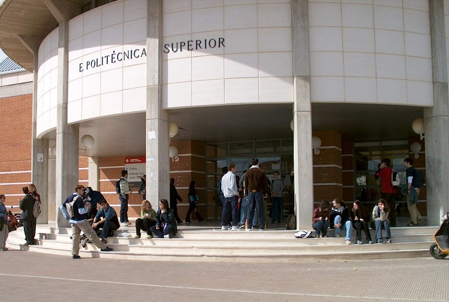
\includegraphics[width=10cm]{figs/esiiab.png}
\end{center}
\caption[Escuela Superior de Ingeniería Informática I]{Escuela Superior de Ingeniería Informática. Esto es un texto descriptivo algo más largo que puede producir un efecto feo.}
\label{fig:esiiabI}
\end{figure}



\begin{figure}[p] 
\captionsetup{width=0.8\linewidth}
\begin{center}
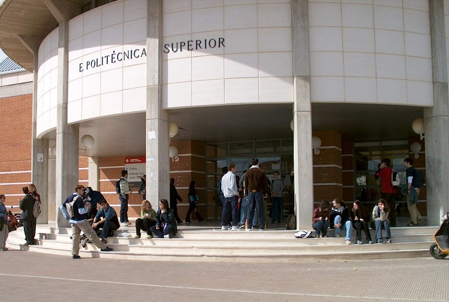
\includegraphics[width=10cm]{figs/esiiab.png}
\end{center}
\caption[Escuela Superior de Ingeniería Informática II]{Escuela Superior de Ingeniería Informática. Esto es un texto descriptivo algo más largo que puede producir un efecto feo.}
\label{fig:esiiabII}
\captionsetup{width=0.9\linewidth}
\end{figure}

Se incluye el paquete \verb+subfigure+ para la inclusión de figuras con varias imágenes o gráficas, como la que muestra la figura \ref{fig:subfiguras}.
\begin{figure}[htb]
\begin{center}
\begin{subfigure}[b]{0.4\linewidth}
\begin{center}
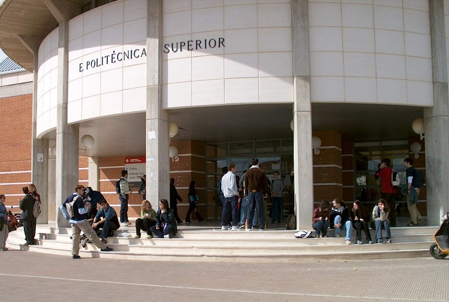
\includegraphics[width=0.9\linewidth]{figs/esiiab.png}
\caption{Fotografía de la izquierda}\label{fig:esiiabIII}
\end{center}
\end{subfigure} 
\begin{subfigure}[b]{0.4\linewidth}
\begin{center}
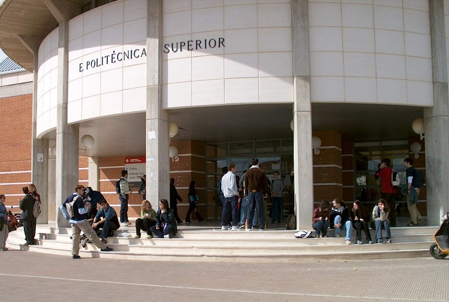
\includegraphics[width=0.9\linewidth]{figs/esiiab.png}
\caption{Fotografía de la drecha}\label{fig:esiiabIV}
\end{center}
\end{subfigure} 
\end{center}
\caption[Ejemplo de subfiguras]{Ejemplo de inclusión de subfiguras}
\label{fig:subfiguras}
\end{figure}



\section{Algorithms and code}

Con respecto a los algoritmos (pseudocódigo) y código pueden implementarse, respectivamente, mediante el uso de los paquetes \verb+algorithmic+ y \verb+listings+. Pueden configurarse ambos entornos el archivo \verb+include\configuracion+. Por otra parte, se han definido dos entornos flotantes, denominados \verb+algorithm+ y \verb+code+ para encapsular y mostrar ambos tipos de elemento de manera uniforme.\\


El algoritmo \ref{alg:search} muestra un ejemplo de pseudocódigo. Se han añadido dos comandos, \verb+\va{variable}+ para distinguir las \va{variables}, y \verb+\fu{funcion}+ para distinguir las \fu{Funciones}. \\



\begin{algorithm}[b]
\begin{algorithmic}[1]
 	\Function{Tree-Search}{ }
 	\State \va{open} $\leftarrow$ \Call{CreateNode}{\fu{Initial-State}} \Comment{Creates the root}
	\While {\va{open} $\neq \emptyset$}
		\State \va{node} $\leftarrow$ \Call{Extract}{\va{open}}
		\If {\Call{TestGoal}{\va{node.STATE}}}
			\State \Return \Call{RecoverPath}{\va{node}} \Comment{Solution found}
		\EndIf		
				
		\State \va{successors} $\leftarrow$ \Call{Expand}{\va{node}}
		\ForAll {\va{successor} \bft{en} \va{successors}} \Comment{Processes each successor }
			\State  \Call{Insert}{\va{successor, open}}
		\EndFor	
	\EndWhile
	\State \Return failure \Comment{No solution have been found}
 	\EndFunction
\end{algorithmic}
\caption{Tree-Search exploration}
\label{alg:search}
\end{algorithm}

Por último, el listado \ref{alg:code} muestra el código del algoritmo \ref{alg:search} en \textit{Python}. El paquete \verb+listings+  contiene multitud de opciones para el manejo de distintos lenguajes y para personalización.

\begin{code}
\begin{lstlisting}

def search(initial):
	open = [initial]
	while open:
		node = open.pop()
		if testGoal(node):
			return recoverPath(node)
		successors = expand(node)
		for succesor in successors:
			open.append(succesor)
	return failure
		
\end{lstlisting}
\caption{Ejemplo de código en Python}
\label{alg:code}
\end{code}


\section{Bibliography}

Esto es una cita \cite{RUSSELL} y esto otra \cite{AlphaZero}. La bibliografía se gestiona con bibtex y un estilo predefinido. No se han hecho modificaciones de momento.

\section{Mathematical notation}

Utiliza las fuentes por defecto del tema, aunque también se pueden cambiar.

\[
J(\theta)=\frac{1}{2m}\left[ \sum_{i=1}^m\left(h_\theta(x^{(i)})-y^{(i)}\right)^2 + \lambda \sum_{j=1}^n \theta_j^2 \right], \mbox{ } \lambda >0
\]

 

% Utilidades para anotaciones
\chapter{Marks and help}

Se han introducido algunos elementos que permiten dejar marcas para indicar que algunas cosas provisionales se han de corregir. Por ejemplo \verb+\pcite+ deja esta señal \pcite para indicar que se ha de añadir una cita bibliográfica en un punto concreto. \\

\ps

Las marcas \verb+\ps+ y \verb+\fs+ permiten marcar y delimitar un bloque con contenido provisional, y que debe ser revisado posteriormente.

\fs \\


Existen métodos más avanzados para hacer anotaciones, como los que ofrece \verb+todonotes+. Permiten insertar notas al margen \todo{Como por ejemplo ésta.}.  \\

También  permite utilizar notas en el propio texto.  \todo[inline]{En internet hay combinaciones de colores interesantes para destacar distintos tipos de notas}  


\section{Figures}

Este paquete tiene otros comandos como \verb+\missingfigure+ para indicar que faltan figuras. \\

\missingfigure{Aquí se puede escribir la descripción de la figura que falta} 

% -------------------------------
% Apéndices
% -------------------------------
\appendix
\chapter{Annex 1}
\lipsum[1-2]

\cleardoublepage
\thispagestyle{empty}


% -------------------------------
% Bibliografía
% -------------------------------
\bibliographystyle{apalike}
\bibliography{bib/ref} 
\addcontentsline{toc}{chapter}{Bibliography} 

\end{document}